\documentclass[12pt]{article}
\usepackage{pgf, tikz}
\usepackage{amsmath, amsfonts, amssymb, graphicx}
\usepackage{float}
\usepackage[utf8]{inputenc}
\usepackage[spanish]{babel}
\usepackage{amsthm}
\usepackage{caption}
\usepackage{subcaption}

\setlength{\textheight}{23cm} \setlength{\evensidemargin}{0cm}
\setlength{\oddsidemargin}{-.5cm} \setlength{\topmargin}{-3cm}
\setlength{\textwidth}{17.5cm} \setlength{\parskip}{.2cm}


%opening

\begin{document}
	\begin{picture}(80, 80)
	\put(170,0){\hbox{
\includegraphics[scale=0.6]{cimat_logo.png}}}
	\end{picture}
	
	\begin{center}
		\begin{huge}
			Centro de Investigación en Matemáticas, A.C.
		\end{huge}
	\end{center}

	\begin{center}
		\begin{large}
			Descripción tarea 9 - Métodos numéricos
		\end{large}
	\end{center}
	
	\begin{center}
		\textbf{Erick Salvador Alvarez Valencia}
	\end{center}

	\begin{center}
		26 de Octubre de 2017
	\end{center}



%\maketitle

%\tableofcontents

\section{Introducción}
En el presente reporte se describirán tres métodos de interpolación de puntos, los cuales se enfocan en generar los coeficientes de el polinomio que pasará por el conjunto de puntos dado. Se describirá a grandes rasgos en qué consiste cada método, un ejemplo de ejecución, y al finalizar se mostrarán los pasos para compilar y ejecutar cada uno de los programas.

\section{Interpolación polinomial}

\subsection{Descripción}
Se tiene un conjunto de n + 1 puntos distintos $\{(x_i, y_i)\}_{i=0}^n$ y se quiere encontrar un polinomio de grado m a lo mucho que pase por ellos tal que $p_m(x_i) = y_i$. Una idea es construir un polinomio de grado m = n + 1 que sea combinación lineal de las abscisas y que su resultado sea una de las ordenadas por las que se quiere interpolar.

$$p_m(x_i) = a_mx_i^m + a_{m-1}x_i^{m-1} + ... + a_1x_i + a_0 = y_i$$

Al hacer esto para cada $y_i$ obtendremos un sistema de $(n + 1) * (n + 1)$ ecuaciones, que al resolverlo podremos conocer el valor de los coeficientes $a_i$ del polinomio interpolador.

\subsection{Ejemplo de ejecución}
A continuación se mostrará el resultado de la ejecución del método de interpolación polinomial con un conjunto de 7 puntos, a su vez se adjuntarán las gráficas generadas para ver qué tan buena fue la aproximación.\\

\begin{figure}[h!]
	\centering
	\begin{subfigure}{0.6\textwidth}
		\centering
		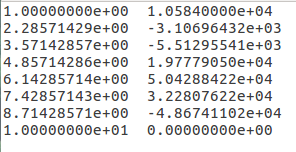
\includegraphics[width=.4\linewidth]{E1.png}
		\caption{Puntos iniciales.}
	\end{subfigure}%
	\begin{subfigure}{0.5\textwidth}
		\centering
		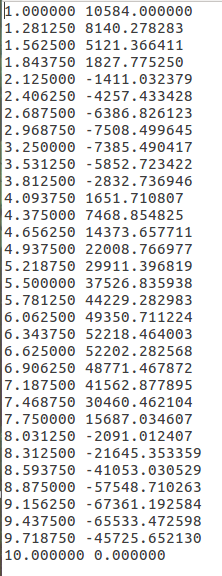
\includegraphics[width=.4\linewidth]{E2.png}
		\caption{Puntos de interpolación.}
	\end{subfigure}
	\caption{Tablas de puntos para la interpolación polinomial.}
\end{figure}

En la Figura 1. podemos observar que la discretización generada en el intérvalo $[x_1, x_n]$ pasa de manera muy cercana a los puntos propuestos en la tabla 1.a.\\

\begin{figure}[h!]
	\centering
	\begin{subfigure}{0.8\textwidth}
		\centering
		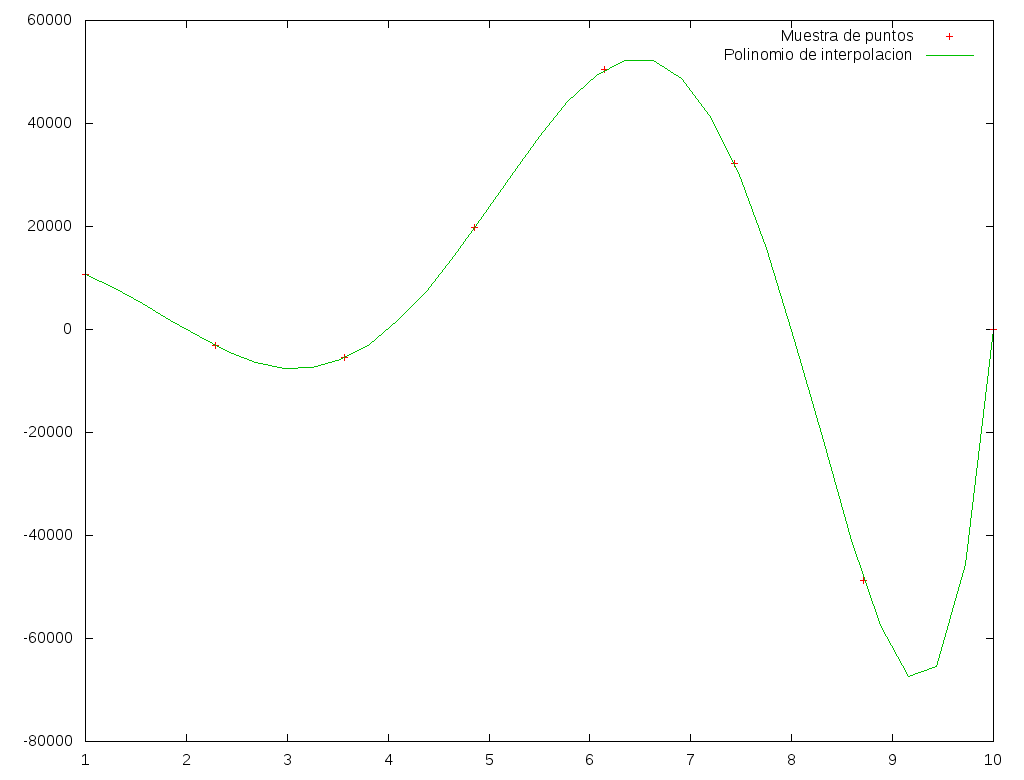
\includegraphics[width=.4\linewidth]{Grafica1.png}
		\caption{Puntos iniciales.}
	\end{subfigure}
	\caption{Tablas de puntos para la interpolación polinomial.}
\end{figure}

\section{Polinomios de Lagrange}
\subsection{Descripción}
Una base polinómica de Lagrange se define de la siguiente manera: $l_{j}(x) = \prod_{j=0, j \neq i}^{n}\frac{x - x_j}{x_i - x_j}$ Si se tiene una serie de puntos distintos $x_0,x_1,...,x_n$ y $f(x)$ es una función cuyos valores están dados en esos puntos por $f(x_0),f(x_1),...,f(x_n)$ entonces existe un único polinomio $L(x)$ de grado al menos $n$ con la propiedad siguiente: $f(x_k) = L(x_k),\ k=0,1,2,...n$ donde el polinomio $L(x)$ es una combinación lineal de las bases polinómicas de Lagrange: $L(x) = \sum_{j = 0}^{k} = y_jl_j(x)$. Se puede demostrar que las bases polinómicas de Lagrange son una base del espacio de los polinomios, de esta forma se garantiza la existencia de $L(x)$.\\

Para este programa se leyeron los $(n + 1)$ puntos y se calculó el polinomio $p_n(x)$ como la combinación lineal de las bases polinómicas de Lagrange donde los coeficientes de la combinación venían siendo representados por los valores de las abscisas de los puntos.

\subsection{Ejemplo de ejecución}
A continuación se mostrará el resultado de la ejecución del método de interpolación por polinomios de Lagrange con un conjunto de 7 puntos.\\

\begin{figure}[H]
	\centering
	\begin{subfigure}{0.6\textwidth}
		\centering
		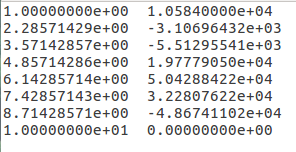
\includegraphics[width=.3\linewidth]{E1.png}
		\caption{Puntos iniciales.}
	\end{subfigure}%
	\begin{subfigure}{0.5\textwidth}
		\centering
		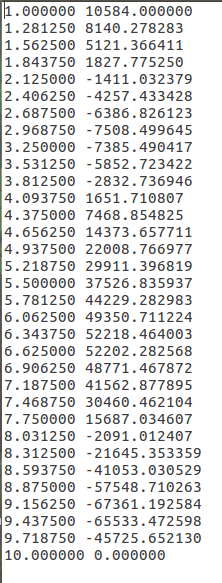
\includegraphics[width=.3\linewidth]{E3.png}
		\caption{Puntos de interpolación.}
	\end{subfigure}
	\caption{Tablas de puntos para la interpolación de Lagrange.}
\end{figure}

Podemos ver que para el conjunto de puntos usado en el método de interpolación polinomial, este método nos arroja exactamente el mismo conjunto de puntos de interpolación, claro que hay que mencionar que la discretización se hizo de la misma forma. Por lo anterior, se puede ver que la gráfica que se generaría sería la misma, por lo que se omitirá.

\section{Polinomio de Newton de diferencias dividias}
El método de interpolación mediante diferencias divididas es un método de construcción de polinomios interpoladores que utiliza un esquema recursivo. Se considera a $P_n(x)$ un polinomio de grado al menos $n$, que se aproxima con la función $f(x)$ en los puntos distintos $x_0, x_1, ..., x_n$. Las diferencias divididas de $f(x)$ respecto a estos puntos pueden ser obtenidas demostrando que $P_n(x)$ viene definido por:

$$P_n(x) = a_0+a_1(x-x_0)+a_2(x-x_1)+...+a_n(x-x_0)...(x-x_{n-1})$$

en donde $a_0,a_1,...,a_n$ son los coeficientes polinomioales. Para este método hay que aplicar un algoritmo que calcule los términos de las diferencias divididas, las cuales denotamos por:

$$f[x_i,x_j]=\frac{f[x_j] - f[x_i]}{x_j - x_i}$$

Vemos que hay una relación recursiva en ellas, por lo cual podemos ir guardando las que ya se calcularon en una tabla y posteriormente usarlas para calcular las próximas. Encontraremos el polinomio interpolador como una combinación lineal del polinomio de Newton y de los coeficientes que serán las diferencias divididas.

$$P_n(x) = \sum_{i=0}^{n}a_{0,i} \prod_{j=0}^{i-1}(x-x_j)$$

Donde $a_{0,i}$ era la i-ésima columna de la matriz de diferencias dividias.

\subsection{Ejemplo de ejecución}
A continuación se mostrará el resultado de la ejecución del método de interpolación por polinomios de Newton con un conjunto de 7 puntos.\\

\begin{figure}[H]
	\centering
	\begin{subfigure}{0.6\textwidth}
		\centering
		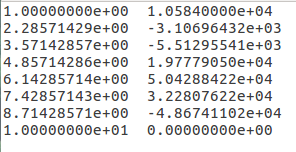
\includegraphics[width=.3\linewidth]{E1.png}
		\caption{Puntos iniciales.}
	\end{subfigure}%
	\begin{subfigure}{0.5\textwidth}
		\centering
		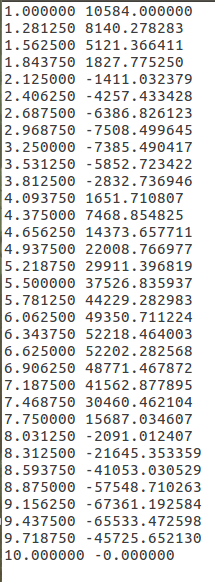
\includegraphics[width=.3\linewidth]{E4.png}
		\caption{Puntos de interpolación.}
	\end{subfigure}
	\caption{Tablas de puntos para la interpolación de Newton.}
\end{figure}

Al igual que en los dos métodos anteriores, este método de interpolación volvió a generar la misma tabla de puntos y por ende la misma gráfica.
Podríamos ver diferencias en estos métodos con usando un conjunto de puntos inicial más grande, ya que con el método de interpolación polinomial la matriz se va mal condicionando y el método de Lagrange requiere muchas operaciones matemáticas.

\section{Compilación y ejecución}
Para esta tarea, los programas se dividieron en tres carpetas, mediante las cuales se encuentran los archivos del código y los de prueba, hay que mencionar que para cada programa se usará la misma forma de compilar, por lo que solo es necesario describir los pasos una vez.\\

\textbf{Para compilar:} En la carpeta encontraremos los archivos $.c$ y $.h$ con los que se podrá compilar el ejecutable. De la misma forma, en conjunto con los archivos anteriores, también podremos encontrar un Makefile para, en caso de encontrarse en linux, compilar de manera sencilla.

\begin{enumerate}
	\item \textbf{Compilar usando Makefile:} En la terminal, nos colocamos en el directorio donde se encuentre el programa, y ejecutamos el comando $make$, automáticamente se realizará la compilación y se generará el ejecutable. El Makefile también contiene el comando $make\ clean$ el cual limpiará los archivos generados por la compilación, incluyendo el ejecutable.
	\item \textbf{Compilar directamente:} De la misma forma, podemos compilar directamente usando los siguientes comandos (en terminal):
	\begin{itemize}
		\item gcc -c main.c -o obj/main.o
		\item gcc -c memo.c -o obj/memo.o
		\item gcc -c reader.c -o obj/reader.o
		\item gcc -c matriz\_vector.c -o obj/matriz\_vector.o
		\item gcc -c met\_num.c -o obj/met\_num.o
		\item gcc -o main obj/main.o obj/memo.o obj/reader.o obj/matriz\_vector.o obj/met\_num.o\ -lm
	\end{itemize}
\end{enumerate}

\textbf{Para ejecutar:} Únicamente debemos de usar el comando $./main$ para ejecutar el programa en consola, este recibe un argumento:
\begin{itemize}
	\item \textbf{Un string:} El nombre del archivo binario donde se encuentra la matriz de puntos.
\end{itemize}

El programa ejecutará el método de interpolación polinomial con los puntos iniciales y generará un archivo de texto que contendrá los puntos discretos obtenidos evaluando el polinomio interpolador.
\end{document}
